\documentclass[11pt]{article}

\usepackage[margin=1in]{geometry}
\usepackage{amsmath,amssymb,booktabs,graphicx,xcolor}
\usepackage[colorlinks=true,allcolors=blue!55!black]{hyperref}

\newcommand{\floor}[1]{\left\lfloor #1\right\rfloor}
\newcommand{\ceil}[1]{\left\lceil #1\right\rceil}
\newcommand{\KT}{d_{\mathrm{KT}}}

\title{\textbf{Fair Rankings That Still Work After One Candidate Is Removed}\\
\large}
\author{Andy Zhuang}
\date{August 30, 2026}

\begin{document}
\maketitle

\begin{abstract}
Sometimes a ranking is fair at first, but it stops being fair after one
candidate is removed.  This paper studies a simple version with two groups.
We want the first $k$ positions to have about the right number of candidates
from each group for every $k$, even after any one candidate is deleted.  We
call this \emph{removal-robust fairness}.  Our main result is that a robust
ranking always exists for two groups.  We give one method that builds it from
left to right, with work that grows in direct proportion to the number of
candidates.  We also give a table-based method that changes one input ranking
as little as possible.  For several inputs, a known idea gives an answer whose
cost is at most three times the best possible robust cost.  Some small computer
tests show that a p-fair ranking does not always stay p-fair after a removal.
\end{abstract}

\section{Introduction}

Rank aggregation means taking several rankings and making one final ranking.
For example, a few teachers could rank scholarship applicants, and the school
needs one list at the end.  The Kemeny idea is to choose a final list that has
as few pair disagreements as possible with the input lists.  This problem is
already hard to solve exactly.

There can also be groups that should be represented near the top of the list.
Wei et al.~\cite{wei2022} studied proportionately fair rank aggregation.  A
\emph{prefix} of length $k$ means the first $k$ positions.  If group $A$ has
$a$ of the $n$ candidates, its exact share in this prefix is $ka/n$.  This
number might not be a whole number, so we allow it to be rounded down or up.
A ranking is proportionately fair when this rule works for every $k$.

But real lists can change.  A student accepts another offer, or a job
candidate becomes unavailable.  If that person is just crossed off, the
percent of the two groups changes.  The old fairness proof might not work.
Recomputing the whole list can also move people who did nothing, which is not
always easy to explain.

Here is a small example.  Let $A$ and $B$ be the two group labels.  There are
three $A$'s and five $B$'s in
\[
  B\ B\ A\ B\ B\ A\ B\ A.
\]
This pattern is fair.  If the $A$ in position 3 is removed, the first four
remaining positions are all $B$.  Now there are two $A$'s out of seven people,
so a prefix of length four should have at least
$\floor{4\cdot2/7}=1$ member of $A$.  It has zero.  This is why just being fair
the first time is not enough.

So, our question is:

\begin{quote}
Can we publish one fair ranking that stays fair after any single person is
removed, without rearranging everybody else?
\end{quote}

In this paper, we only study two groups and one removal.

\section{Definitions in a simple form}

\medskip
\noindent\textbf{Definition (ranking).}
A \emph{ranking} is a strict ordering $\pi=(v_1,\ldots,v_n)$ of a number of candidates.
\medskip

\noindent\textbf{Definition (group pattern).}
Suppose every candidate belongs to exactly one of the groups
$G_1,G_2,\ldots,G_\ell$.  Read a ranking from first place to last place and
write down only the group label of each candidate.  This list of labels is the
\emph{group pattern}.  More formally, if $g(v_j)$ is the group of the
candidate in position $j$, then the group pattern of
$\pi=(v_1,\ldots,v_n)$ is
\[
 \gamma(\pi)=\bigl(g(v_1),\ldots,g(v_n)\bigr)
 \in\{G_1,\ldots,G_\ell\}^n.
\]
The last notation only says that there are $n$ labels and that each label is
one of $G_1,\ldots,G_\ell$.  The candidate names are not kept.
\medskip

\noindent\textbf{Definition (binary group pattern).}
A group pattern is a \emph{binary group pattern} when there are exactly two
groups.  In this case,
\[
 \gamma(\pi)\in\{G_1,G_2\}^n.
\]
Thus ``binary'' means that the sequence uses two group labels.

A ranking gives exactly one group pattern, but different rankings can have
the same group pattern.  For example, the pattern $A,B,A$ does not say which
$A$-candidate is first.  If we also choose an order for the candidates inside
each group, then the pattern tells us where to put every candidate.
\medskip

The rest of this paper studies the binary case.  We rename $G_1$ as $A$ and
$G_2$ as $B$.
To make it simple, we call a binary group pattern a \emph{binary
pattern}.  Suppose $A$ has $a$ candidates and $B$ has $b=n-a$.  For
counting purposes, define
\[
 x_j=
 \begin{cases}
  1,&\text{if the label in position $j$ is $A$},\\
  0,&\text{if the label in position $j$ is $B$},
 \end{cases}
 \qquad
 c(k)=\sum_{j=1}^{k}x_j.
\]
Thus $c(k)$ is the number of $A$ labels in the first $k$ positions.  The
$0/1$ values are only for counting; the binary pattern itself is the
sequence of two group labels.
For a list with $N$ candidates, including $q$ from group $A$, the exact share
of $A$ in the first $k$ positions is $kq/N$.  We allow this number rounded
down or rounded up.  We use the following shorter notation for these choices:
\[
  W(N,q,k)=
  \left[\floor{\frac{kq}{N}},\ceil{\frac{kq}{N}}\right]\cap\mathbb Z.
\]
Here $\mathbb Z$ means the whole numbers.  Thus $W(N,q,k)$ contains one or two
allowed counts.  The letter ``p'' stands for ``proportionately.''  A pattern
is \emph{p-fair} when
\[
  c(k)\in W(n,a,k) \qquad\text{for every }k=1,\ldots,n.
\]
We do not need a separate test for $B$.  Its count is $k-c(k)$, so an allowed
rounded count for $A$ also gives an allowed rounded count for $B$.  A ranking
is p-fair when its group pattern is p-fair.

\medskip
\noindent\textbf{Definition (removal-robustness).}
Let $\pi$ be a p-fair ranking.  For a candidate $v$, let $\pi-v$ be the
ranking made by deleting $v$ and keeping the relative order of every
remaining candidate unchanged.  We call $\pi$ \emph{removal-robust} if
$\pi-v$ is p-fair for every possible candidate $v$.  Fairness after the
removal uses the new list size $n-1$ and the new number of $A$ candidates:
it is $a-1$ when $v$ is from $A$, and it stays $a$ when $v$ is from $B$.

A p-fair binary group pattern is removal-robust when the same condition holds
after deleting any one of its positions.  Therefore, a ranking is
removal-robust exactly when its group pattern is removal-robust.
\medskip

\noindent\textbf{Definition (Kendall distance).}
Let $\pi$ and $\rho$ be two rankings of the same candidate set $C$, where
$|C|=n$.  Look at every pair of candidates.  Count the pair when one ranking
puts the two candidates in one order and the other ranking puts them in the
opposite order.  The total is their \emph{Kendall distance}.  To write this
formally, let $u\prec_\pi v$ mean that $u$ appears before $v$ in $\pi$.
Also, $C^2$ means all ordered pairs chosen from $C$.  Then
\[
 \KT(\pi,\rho)
 =\left|\left\{(u,v)\in C^2:
 u\ne v,\ u\prec_\pi v,\text{ and }v\prec_\rho u\right\}\right|.
\]
It is between 0 and
$\binom{n}{2}=n(n-1)/2$, the total number of candidate pairs.

For example, consider the rankings
\[
 \pi=(a,b,c,d,e)
 \quad\text{and}\quad
 \rho=(b,a,c,e,d).
\]
Only the pairs $\{a,b\}$ and $\{d,e\}$ are reversed, so
$\KT(\pi,\rho)=2$.  With five candidates, the largest possible Kendall
distance is $\binom{5}{2}=10$.

\medskip
\noindent\textbf{Definition (Kemeny cost).}
Let $P=(\pi_1,\ldots,\pi_m)$ be a profile of $m$ input rankings of the same
set of $n$ candidates.  For an output ranking $\sigma$ of these candidates,
its \emph{Kemeny cost} with respect to $P$ is
\[
 \operatorname{cost}_P(\sigma)
 =\sum_{i=1}^{m}\KT(\sigma,\pi_i).
\]
When the profile is clear, we write this as $\operatorname{cost}(\sigma)$.
Here $m$ is the number of input rankings, while $n$ is the number of
candidates in each ranking.
\medskip

\section{Checking Whether a Pattern Is Removal-Robust}

\medskip
\noindent\textbf{Lemma.}
Given a binary pattern with $n$ positions and $a$ members of group $A$, we
can determine whether it is removal-robust in $O(n)$ time.
\medskip

\noindent\textit{Proof.}
It sounds like we need to delete every candidate separately and then check
every new prefix.  There is a faster way.  Let $c(k)$ be the old number of
$A$ labels in the first $k$ positions.  Fix a prefix of length $k$ after a
deletion.  If the removed candidate was in an old position after $k$, we say
it was below the prefix.  The new prefix is then the old first $k$ positions.
If the candidate was in one of the old positions $1,\ldots,k$, we say it was
inside the prefix.  The new prefix then comes from the old first $k+1$
positions, with the removed candidate missing.

This makes four cases:

\begin{center}
\begin{tabular}{@{}llll@{}}
\toprule
Removed group & Where it was & New number of $A$ & Fair window \\
\midrule
$A$ & below the prefix & $c(k)$ & $W(n-1,a-1,k)$ \\
$B$ & below the prefix & $c(k)$ & $W(n-1,a,k)$ \\
$A$ & inside the prefix & $c(k+1)-1$ & $W(n-1,a-1,k)$ \\
$B$ & inside the prefix & $c(k+1)$ & $W(n-1,a,k)$ \\
\bottomrule
\end{tabular}
\end{center}

A row only has to be checked when a candidate of that kind and location
actually exists.  For example, the first row matters when $c(k)<a$, since
then an $A$ is still below the prefix.  The third row matters when $c(k)>0$.
For $B$, the second row matters when $k-c(k)<n-a$, and the fourth row matters
when $k-c(k)>0$.

Every deletion and every new prefix fits one of these four rows.  Therefore,
if all four applicable rows pass, every removal passes.  If a row fails, its
corresponding removal also fails.  For each prefix length $k$, there are at
most four checks.  We do this for the $n-1$ possible new prefix lengths and
also check the original pattern.  The work is at most a fixed number of steps
times $n$.  This is what $O(n)$ time means here. \hfill\(\square\)

\section{Existence of robust binary pattern}

The most important result is the following.

\medskip
\noindent\textbf{Theorem.}
Let $n\ge1$ be the total number of candidates.  Suppose group $A$ has $a$
candidates and group $B$ has $n-a$ candidates, where $0\le a\le n$.  Then
there exists a removal-robust p-fair binary pattern, and it can be constructed in $O(n)$ time.
\medskip

\noindent\textit{Proof.}
The cases $a=0,n$ are obvious because everybody has the same label.  The
cases $a=1,n-1$ are also easy: the one different candidate can go in any
position.  Now suppose each group has at least two candidates.

Next, we explain where the five numbers in the proof come from.  Fix a
position $j$ and ask how many $A$ labels are allowed in the first $j$
positions.  Each fairness rule starts with an ideal fraction.  We call this
fraction its \emph{target}.  The rule then allows the target rounded down or
rounded up.  Before any removal, p-fairness says
\[
 c(j)\in W(n,a,j),
\]
so its target number is
\[
 T_0=\frac{ja}{n}.
\]
For the two ``below the prefix'' rows from the last section, let $k=j$.
If an $A$ is removed below, then
\[
 c(j)\in W(n-1,a-1,j),
 \qquad T_{A\downarrow}=\frac{j(a-1)}{n-1}.
\]
If a $B$ is removed below, the $A$ total stays equal to $a$, so
\[
 c(j)\in W(n-1,a,j),
 \qquad T_{B\downarrow}=\frac{ja}{n-1}.
\]

The two ``inside the prefix'' rows are a little different.  We should let $k=j-1$
because, after an inside removal, the new first $j-1$ people came from the
old first $j$ people.  Removing a $B$ does not change the number of $A$s, so
\[
 c(j)\in W(n-1,a,j-1),
 \qquad T_{B\mathrm{in}}=\frac{(j-1)a}{n-1}.
\]
Removing an $A$ changes the new count to $c(j)-1$.  So
\[
 c(j)-1\in W(n-1,a-1,j-1).
\]
Adding 1 back to both allowed rounded values gives us:
\[
 c(j)\in
 \left\{1+\floor{\frac{(j-1)(a-1)}{n-1}},
             1+\ceil{\frac{(j-1)(a-1)}{n-1}}\right\},
 \qquad
 T_{A\mathrm{in}}=1+\frac{(j-1)(a-1)}{n-1}.
\]

So the original p-fairness rule and the four removal cases give five target
numbers:
\[
 T_0,\quad T_{A\downarrow},\quad T_{B\downarrow},\quad
 T_{A\mathrm{in}},\quad T_{B\mathrm{in}}.
\]

The arrow $\downarrow$ means that the removed candidate was below the prefix,
and ``in'' means that the candidate was removed inside it.  For example, if
$n=8$, $a=3$, and $j=4$, the five targets are
\[
  1.5,\quad \frac87,\quad \frac{12}7,\quad
  \frac{13}7,\quad \frac97.
\]
They are all between 1 and 2, so every one of their rounded choices includes
either 1 or 2.  This example shows the main idea of the proof.

Each target $T$ allows the whole numbers from $\floor{T}$ to $\ceil{T}$.  To
make one simple construction, we use both inside targets from $j=2$ onward
and both below targets through $j=n-2$.  Sometimes one of these checks is
stronger than we really need, but an extra fairness check cannot make the
final pattern unsafe.  At $j=n-1$, the only old position below the prefix is
the last position.  For the main case $2\le a\le n-2$, we decide that this
last label will be $B$, so we keep only $T_{B\downarrow}$ there.  This target
will force $c(n-1)=a$, which really does make the last label $B$.  We could
swap $A$ and $B$ to get the other version.

We now look for a whole number accepted by every target being used.  Each
target has a lower rounded value and an upper rounded value.  The largest
lower value and the smallest upper value are
\[
 L(j)=\max_T\floor{T},\qquad
 U(j)=\min_T\ceil{T},
\]
where the maximum and minimum are over the targets used at position $j$.  Any
whole number from $L(j)$ to $U(j)$ passes all of their checks.  We call this
overlap the \emph{common interval}.

Here is why this common interval is never empty.  First take an interior
position $2\le j\le n-2$, where all five targets are used.  We first compare
four of them with $T_0$.  For the first subtraction, using the same
denominator gives
\[
\begin{aligned}
 T_0-T_{A\downarrow}
 &=\frac{ja}{n}-\frac{j(a-1)}{n-1}\\
 &=\frac{ja(n-1)-jn(a-1)}{n(n-1)}\\
 &=\frac{j(n-a)}{n(n-1)}.
\end{aligned}
\]
The other subtractions work in the same way:
\begin{align*}
 0\le T_0-T_{A\downarrow}
   &=\frac{j(n-a)}{n(n-1)}
     \le\frac{(n-2)^2}{n(n-1)}<1,\\
 0\le T_{B\downarrow}-T_0
   &=\frac{ja}{n(n-1)}
     \le\frac{(n-2)^2}{n(n-1)}<1,\\
 0\le T_0-T_{B\mathrm{in}}
   &=\frac{a(n-j)}{n(n-1)}
     \le\frac{(n-2)^2}{n(n-1)}<1,\\
 0\le T_{A\mathrm{in}}-T_0
   &=\frac{(n-a)(n-j)}{n(n-1)}
     \le\frac{(n-2)^2}{n(n-1)}<1.
\end{align*}
Since $2\le a,j\le n-2$, the numbers $a$, $j$, $n-a$, and $n-j$ are all at
most $n-2$.  Also $(n-2)^2<n(n-1)$.  This explains the ``less than 1'' part
of all four lines.
So
\[
 T_{A\downarrow}\le T_0\le T_{B\downarrow}
 \quad\hbox{and}\quad
 T_{B\mathrm{in}}\le T_0\le T_{A\mathrm{in}}.
\]
This tells us that the largest of the five targets must be either
$T_{B\downarrow}$ or $T_{A\mathrm{in}}$, and the lowest must be either
$T_{A\downarrow}$ or $T_{B\mathrm{in}}$.  There are two choices for the
largest and two for the smallest, so there are four possible
largest-minus-smallest differences.  We check all four:
\begin{align*}
 T_{B\downarrow}-T_{A\downarrow}
   &=\frac{j}{n-1}
     \le\frac{n-2}{n-1}<1,
 &T_{B\downarrow}-T_{B\mathrm{in}}
   &=\frac{a}{n-1}
     \le\frac{n-2}{n-1}<1,\\
 T_{A\mathrm{in}}-T_{A\downarrow}
   &=\frac{n-a}{n-1}
     \le\frac{n-2}{n-1}<1,
 &T_{A\mathrm{in}}-T_{B\mathrm{in}}
   &=\frac{n-j}{n-1}
     \le\frac{n-2}{n-1}<1.
\end{align*}
For completeness, here are the last two pairs that have not appeared yet.
They also differ by less than 1:
\begin{align*}
 \left|T_{A\downarrow}-T_{B\mathrm{in}}\right|
   &=\frac{|a-j|}{n-1}
     \le\frac{n-4}{n-1}<1,\\
 \left|T_{B\downarrow}-T_{A\mathrm{in}}\right|
   &=\frac{|a+j-n|}{n-1}
     \le\frac{n-4}{n-1}<1.
\end{align*}
Five numbers have $5\cdot4/2=10$ different pairs.  We have now checked all
ten.  The four largest-minus-smallest checks are the ones the proof really
needs.  They show that, if $H$ is the highest target and $S$ is the lowest,
then $H-S<1$.

The simple idea is that all five targets are squeezed into a space shorter
than 1, so their rounded choices must share a whole number.  To show this
carefully, choose $z=\ceil{S}$, the first whole number at or above $S$.  For
every target $T$ being used, we have $S\le T\le H<S+1$.  The first inequality
gives $z=\ceil{S}\le\ceil{T}$.  Also $T<S+1\le z+1$, which gives
$\floor{T}\le z$.  Therefore
\[
 \floor{T}\le z\le\ceil{T}
\]
for every target at the same time.  In other words,
$L(j)\le z\le U(j)$, so the common interval contains a whole number and cannot
be empty.

The edge positions are simpler.  At $j=1$, we use only $T_0$ and the two below
targets.  The below targets are the highest and lowest, and their
difference is $1/(n-1)<1$.  At $j=n-1$, our chosen last $B$ makes
$T_{B\downarrow}=a$.  The other targets being used are between $a-1$ and $a$,
so all their rounded windows also include $a$.  At $j=n$, all valid targets
equal $a$.  Finally, $a=0$ and $a=n$ give constant patterns.  If $a=1$ or
$a=n-1$, the one minority candidate can be put in any position and the same
floor/ceiling check works.

The common intervals give us one way to build a robust pattern.  They do not
have to contain every possible robust pattern.  We start with no positions
and no $A$ labels, so $c(0)=0$.  At each new position, use
\[
  c(j)=\max\{c(j-1),L(j)\}.
\]
As $j$ goes up by one, each target goes up by an amount between 0 and 1.
Therefore its rounded-down value rises by at most one, and its rounded-up
value does not fall.  The same is true for the borders $L(j)$ and $U(j)$.
When the inside checks begin at $j=2$, a direct calculation gives
$L(1)=0$, $L(2)=1$, and $U(1)=U(2)=1$.  Near the end, we only remove checks.
Thus the lower border never jumps upward by more than one, and the upper border
never moves below its earlier value.

Suppose the old count $c(j-1)$ was inside the earlier common interval.  If it
is still at least $L(j)$, we keep the same count.  Otherwise we raise it to
$L(j)$.  The count stays at most $U(j)$ because the upper border did not move
down and the new common interval is not empty.  It rises by either 0 or 1, so
we write $B$ when it stays the same and $A$ when it rises.  At $j=n$, the only
allowed count is $a$, so the pattern has exactly $a$ labels from group $A$.
It passes the original p-fairness check and all four removal checks.

At each position, we calculate at most five targets and make only a few
comparisons.  Therefore the amount of work grows in direct proportion to
$n$, which is $O(n)$ time.
\hfill\(\square\)

Here is the pseudocode.

\begin{verbatim}
MAKE-ROBUST(n, a)
    if a = 0, return B repeated n times
    if a = n, return A repeated n times
    if a = 1, return one A followed by n-1 B's
    if a = n-1, return one B followed by n-1 A's

    c[0] = 0
    for j = 1,...,n
        compute the common interval [L(j), U(j)]
        c[j] = max(c[j-1], L(j))
    for j = 1,...,n
        output A if c[j] - c[j-1] = 1, otherwise output B
\end{verbatim}

\section{Finding the Closest Robust Ranking to One Input}

Fix one input ranking $\rho$.  We want a removal-robust p-fair ranking
$\sigma$ that makes
\[
 \KT(\sigma,\rho)
\]
as small as possible.  In plain words, we want to change as few candidate
pairs as we can.

Fairness only depends on the group pattern.  After choosing the positions for
groups $A$ and $B$, we still have to put the named candidates into those
positions.  The best choice is to keep the candidates from each group in the
same relative order as in $\rho$.

Here is why.  Suppose $u$ and $v$ are in the same group.  Candidate $u$ comes
before $v$ in $\rho$, but $v$ comes before $u$ in $\sigma$.  Swap their
positions in $\sigma$.  The group pattern does not change, because they have
the same label.  Their disagreement with each other disappears.  Candidates
outside the two positions are not affected.  For a candidate between the two
positions, its total number of disagreements with $u$ and $v$ either stays the
same or becomes smaller.  Repeating this swap removes every reversed pair
from the same group.

We next prove a formula for the remaining distance using only prefix counts.

\medskip
\noindent\textbf{Theorem (prefix-count formula).}
Suppose group $A$ has $a$ candidates and group $B$ has $b$ candidates, so
$n=a+b$.  Let $\sigma$ and $\rho$ be rankings of the same candidates.  Assume
that they use the same relative order inside group $A$ and the same relative
order inside group $B$.

Let $c_\sigma(k)$ be the number of $A$-candidates in the first $k$ positions
of $\sigma$.  Define $c_\rho(k)$ in the same way.  Then
\[
  \KT(\sigma,\rho)
  =\sum_{k=1}^{n-1}\left|c_\sigma(k)-c_\rho(k)\right|.
\]
We stop at $n-1$ because both complete rankings have all $a$ candidates from
group $A$.  Thus $c_\sigma(n)=c_\rho(n)=a$, and the term for $k=n$ would be
zero.
\medskip

\noindent\textit{Proof.}
Write the common within-group orders as
\[
 A_1,A_2,\ldots,A_a
 \qquad\text{and}\qquad
 B_1,B_2,\ldots,B_b.
\]
For each $A_i$, let
\[
 p_i^\sigma=\operatorname{pos}_\sigma(A_i)
 \qquad\text{and}\qquad
 p_i^\rho=\operatorname{pos}_\rho(A_i).
\]
In $\sigma$, exactly $i-1$ other $A$-candidates occur before $A_i$.
Therefore exactly $p_i^\sigma-i$ candidates from $B$ occur before $A_i$.
Since the $B$-candidates keep their common order, these are
$B_1,\ldots,B_{p_i^\sigma-i}$.  Similarly, the $B$-candidates before $A_i$
in $\rho$ are $B_1,\ldots,B_{p_i^\rho-i}$.

Therefore $A_i$ forms a reversed pair with exactly
\[
 \left|(p_i^\sigma-i)-(p_i^\rho-i)\right|
 =\left|p_i^\sigma-p_i^\rho\right|
\]
$B$-candidates in the two rankings.  No same-group pair is reversed, so
\begin{equation}
 \KT(\sigma,\rho)
 =\sum_{i=1}^{a}\left|p_i^\sigma-p_i^\rho\right|.
 \tag{1}
\end{equation}

Now imagine drawing a cut just after position $k$ in both rankings.  If
$c_\sigma(k)>c_\rho(k)$, then exactly
\[
 A_{c_\rho(k)+1},\ldots,A_{c_\sigma(k)}
\]
are to the left of the cut in $\sigma$ but to the right of the cut in
$\rho$.  If $c_\rho(k)>c_\sigma(k)$, the same idea works with the two rankings
exchanged.  Therefore
\[
 |c_\sigma(k)-c_\rho(k)|
\]
counts the $A$-candidates that are on different sides of this cut in the two
rankings.

A fixed candidate $A_i$ is on different sides for exactly
$|p_i^\sigma-p_i^\rho|$ choices of $k$.  Adding over all cuts gives
\[
 \sum_{k=1}^{n-1}|c_\sigma(k)-c_\rho(k)|
 =\sum_{i=1}^{a}|p_i^\sigma-p_i^\rho|
 =\KT(\sigma,\rho),
\]
and equation (1) shows that the last expression is the Kendall distance.  This
proves the formula. \hfill\(\square\)

We can use this formula in a table-based algorithm.

\medskip
\noindent\textbf{Theorem (closest robust ranking).}
Given one input ranking $\rho$ of $n$ candidates, we can find a closest
removal-robust p-fair ranking in $O(n)$ time and $O(n)$ space.
\medskip

\noindent\textit{Proof.}
For every prefix length $k$, let
\[
 h(k)=c_\rho(k).
\]
Thus $h(k)$ is the number of $A$-candidates in the first $k$ positions of the
input ranking.

We fill in a table one position at a time.  The table entry $D[k,i]$ means
that we have filled the first $k$ positions and used exactly $i$ candidates
from group $A$.  It stores the smallest cost
\[
 \sum_{t=1}^{k}|c(t)-h(t)|
\]
among the partial patterns that have passed every check we can do so far.  For
each $k$, we create entries only for the one or two counts allowed by
$W(n,a,k)$.  All other pairs $(k,i)$ are treated as unreachable and are not
stored.  We start with $D[0,0]=0$.

From $D[k,i]$, there are at most two choices for position $k+1$.  Adding a
$B$ keeps the $A$ count equal to $i$.  Adding an $A$ changes it to $i+1$.
Suppose the new count is $i'$.  We first check p-fairness at prefix $k+1$.
When $k\ge1$, we now know both
\[
 c(k)=i\qquad\text{and}\qquad c(k+1)=i',
\]
so we can do all four checks from Section~3 for prefix $k$.  If they pass, we
add
\[
 |i'-h(k+1)|
\]
to the cost already stored in $D[k,i]$.

If two partial patterns reach the same entry $D[k,i]$, they have the same
choices later because they have the same prefix length and the same current
count.  We only need to keep the cheaper one.  This is the main reason the
table method works.

Every complete pattern kept by the table is p-fair and passes all four
removal checks for every prefix.  Section~3 says it is removal-robust.  The
reverse is also true: every removal-robust pattern passes those exact checks,
so the table does not miss it.  By the prefix-count formula, the final table
cost is exactly the Kendall distance from $\rho$.  Thus the cheapest final
entry gives a closest robust pattern.

For a fixed prefix length, p-fairness allows at most two possible $A$ counts:
the rounded-down and rounded-up choices.  For each count, we try only the next
labels $A$ and $B$.  Thus we examine at most four choices at each position.
The work grows in direct proportion to $n$, so it is $O(n)$.  We also remember
which earlier table entry gave each cheapest value.  Following these saved
entries backward produces the final pattern and uses $O(n)$ space.

Finally, we fill the $A$ and $B$ positions with candidates in their order
from $\rho$.  This gives the closest full ranking. \hfill\(\square\)

This table method uses the exact four-case test from Section~3.  The common
interval from Section~4 was only used to build one robust pattern and prove
that one always exists.  It can leave out other robust patterns, so we do not
use it when searching for the closest one.

\section{Combining Several Input Rankings}

Suppose we are given the input rankings
\[
 P=(\pi_1,\ldots,\pi_m).
\]
We want one removal-robust p-fair ranking that has the smallest total Kendall
distance from these $m$ inputs.  Checking one pattern is quick, and Section~5
finds the closest robust ranking to one input.  Finding the exact best answer
for several inputs is still hard.  In fact, it is NP-hard.  This means that a
polynomial-time exact algorithm for our problem would also give
polynomial-time algorithms for known NP-hard problems, which would be a major
new result in computer science.

\medskip
\noindent\textbf{Theorem (NP-hardness).}
Finding an exact minimum-cost removal-robust p-fair ranking is NP-hard, even
when there are only two nonempty groups.
\medskip

\noindent\textit{Proof.}
The idea is to begin with a ranking problem that is already known to be hard.
We will add one special candidate and turn it into our problem.  If someone
could solve the new problem exactly, the answer would also solve the old one.
This kind of argument is called a \emph{reduction}.

The old problem is Kemeny rank aggregation without a fairness rule.  Given
rankings $P=(\pi_1,\ldots,\pi_m)$, it asks for a ranking $\sigma$ with the
smallest total Kendall distance
\[
 \operatorname{cost}_P(\sigma)
 =\sum_{i=1}^{m}\KT(\sigma,\pi_i).
\]
There is no p-fairness or removal rule in this old problem, and it is already
known to be NP-hard~\cite{dwork2001}.  Suppose it has $q$ candidates.  Put all
of them in group $A$.  Add one new candidate $d$ in group $B$ and put $d$ at
the end of every input ranking.  Candidate $d$ is only used to connect the two
problems, so we call it a dummy candidate.  We only added one item to every
ranking, so making the new input is quick compared with solving it.

First we show that every possible output ranking is removal-robust and p-fair.
There are $q$ candidates in $A$ and one in $B$.  For a prefix of length
$1\le k\le q$, its number of $A$-candidates is either $k$ or $k-1$, depending
on whether the dummy is in the prefix.  Also,
\[
 k-1 < \frac{kq}{q+1} < k.
\]
Therefore $k-1$ and $k$ are exactly the floor and ceiling choices, so every
placement of the dummy is p-fair.  The full prefix has exactly $q$
$A$-candidates.

If the dummy is removed, every remaining candidate is in group $A$, which is
p-fair.  If an $A$-candidate is removed, there are $q-1$ candidates in $A$
and one in $B$.  For every non-full prefix $1\le k\le q-1$,
\[
 k-1 < \frac{k(q-1)}{q} < k,
\]
so both possible counts, $k-1$ and $k$, are allowed.  In other words, every
output ranking is also removal-robust.  The full prefix is fair too because it
has exactly $q-1$ members of $A$.

Next, we show why a best output must put $d$ last.  Let $\sigma'$ be any
output ranking, and let $\sigma$ be the ranking of the original candidates
made by deleting $d$ from $\sigma'$.  Suppose $s$ original candidates appear
after $d$ in $\sigma'$.  Every input puts all original candidates before $d$,
so each of these $s$ candidates makes one disagreement with $d$ in every one
of the $m$ inputs.  All the other disagreements are between original
candidates.  Therefore
\[
 \operatorname{cost}_{P'}(\sigma')
 =\operatorname{cost}_{P}(\sigma)+ms,
\]
where $P'$ is the new profile containing the dummy candidate.

If $s>0$, moving $d$ to the last position keeps the order $\sigma$ unchanged
and removes all $ms$ of these extra disagreements.  The new ranking is still
allowed because we already showed that every ordering is removal-robust.
Therefore a best output has $s=0$, meaning $d$ is last.  Its cost is then
exactly the Kemeny cost of its ordering of the original candidates.
So if we could solve the new robust problem exactly, deleting $d$ from its
answer would solve the original Kemeny problem without a fairness rule.  Since
that problem is NP-hard, our problem is NP-hard too.
\hfill\(\square\)

Even though finding the exact best combined answer is NP-hard, the method from
Section~5 gives us a simple backup plan:

\begin{enumerate}
  \item Start with each input ranking, one at a time.
  \item Find the closest robust version of that input.
  \item Measure how well each of these versions agrees with all the inputs.
  \item Return the one with the smallest total cost.
\end{enumerate}

We call the Section~5 method \texttt{CLOSEST-ROBUST}.  On input $\pi_i$, it
returns a closest removal-robust p-fair ranking, which we name $\tau_i$.  Thus
$\tau_i$ is the closest robust version of $\pi_i$.  If there is a tie, either
closest ranking can be used.

Here is the full approximation algorithm written in pseudocode.

\begin{verbatim}
ROBUST-AGGREGATE(pi[1], ..., pi[m])
    Input: m rankings of the same n candidates
    Output: one removal-robust p-fair ranking

    best_ranking = NONE
    best_cost = INFINITY

    for i = 1, ..., m
        tau[i] = CLOSEST-ROBUST(pi[i])
        total = 0

        for j = 1, ..., m
            total = total
                    + KENDALL-DISTANCE(tau[i], pi[j])

        if total < best_cost
            best_ranking = tau[i]
            best_cost = total

    return best_ranking
\end{verbatim}

Here \texttt{NONE} means that no ranking has been selected yet, and
\texttt{INFINITY} means a starting cost larger than any real cost.  For each
closest robust version $\tau_i$, the inner loop computes
\[
 \operatorname{cost}_P(\tau_i)
 =\sum_{j=1}^{m}\KT(\tau_i,\pi_j).
\]
The algorithm remembers the $\tau_i$ with the smallest total cost and returns
it.  We call this ranking $\sigma_{\mathrm{out}}$, where ``out'' means the
output.

\medskip
\noindent\textbf{Theorem (approximation guarantee).}
The algorithm returns a removal-robust p-fair ranking whose Kemeny cost is at
most three times the cost of the best removal-robust p-fair ranking.
\medskip

\noindent\textit{Proof.}
Let $\sigma^*$ mean the best possible removal-robust p-fair ranking.  Its cost
is written as
\[
 \mathrm{OPT}=\operatorname{cost}_P(\sigma^*)
 =\sum_{i=1}^{m}\KT(\pi_i,\sigma^*).
\]
The letters OPT stand for this best, or optimal, cost.  At least one input
ranking, call it $\pi_r$, must satisfy
\[
 \KT(\pi_r,\sigma^*)\le \frac{\mathrm{OPT}}{m}.
\]
This is because the left side is one of the $m$ numbers whose sum is
$\mathrm{OPT}$, so at least one of them cannot be bigger than their average.

The ranking $\tau_r$ is a closest robust ranking to $\pi_r$.  The ranking
$\sigma^*$ is also robust, so it gives us a valid comparison.  Therefore
$\tau_r$ cannot be farther from $\pi_r$ than $\sigma^*$ is:
\[
 \KT(\tau_r,\pi_r)\le \KT(\sigma^*,\pi_r).
\]
Kendall distance has a useful rule called the triangle inequality.  It says
that going directly between two rankings is never farther than taking a route
through other rankings.  For any input $\pi_j$, use the route
\[
 \tau_r\longrightarrow\pi_r\longrightarrow\sigma^*\longrightarrow\pi_j.
\]
The triangle inequality gives
\begin{align*}
 \KT(\tau_r,\pi_j)
 &\le \KT(\tau_r,\pi_r)
       +\KT(\pi_r,\sigma^*)
       +\KT(\sigma^*,\pi_j)\\
 &\le 2\KT(\pi_r,\sigma^*)+\KT(\sigma^*,\pi_j).
\end{align*}
Now add this inequality for all $m$ inputs.  The first distance on the last
line appears once for every input, so
\begin{align*}
 \operatorname{cost}_P(\tau_r)
 &\le 2m\KT(\pi_r,\sigma^*)+\operatorname{cost}_P(\sigma^*)\\
 &\le 2m\left(\frac{\mathrm{OPT}}m\right)+\mathrm{OPT}\\
 &=3\mathrm{OPT}.
\end{align*}
Finally, $\tau_r$ is one of the $m$ rankings checked by the algorithm.  The
algorithm returns the checked ranking with the smallest total cost.  Therefore
$\sigma_{\mathrm{out}}$ cannot cost more than $\tau_r$:
\[
 \operatorname{cost}_P(\sigma_{\mathrm{out}})
 \le \operatorname{cost}_P(\tau_r)
 \le 3\mathrm{OPT}.
\]
This is what we mean by a 3-approximation: its cost is no more than three
times the best possible cost.
\hfill\(\square\)

Finding the closest robust version of all $m$ inputs takes $O(mn)$ time,
because each call to \texttt{CLOSEST-ROBUST} takes $O(n)$ time.  We then have
$m$ versions, and each is compared with all $m$ inputs.  This makes $m^2$
Kendall-distance calculations.

To compare two rankings, replace each candidate in the first ranking by its
position in the second ranking.  A reversed candidate pair becomes an
out-of-order pair of numbers, which is called an inversion.  Merge sort can
count these pairs in $O(n\log n)$ time.  Thus the comparisons take
$O(m^2n\log n)$ time, and the whole runtime is
$O(mn+m^2n\log n)$.

The general idea of making a closest fair version of every input and choosing
the cheapest one was already used in fair rank
aggregation~\cite{wei2022,chakraborty2025}.  Here we apply that known idea to
the one-removal condition.

\section{Code and Small Tests}

We wrote a small implementation and tried it on several examples.  The tests
asked three questions:

\begin{enumerate}
  \item Does every p-fair pattern already survive one removal?
  \item How did the robust algorithm's cost compare with a simpler p-fair
        algorithm's cost?
  \item On inputs small enough that we could try every answer, how close was
        our algorithm to the best answer?
\end{enumerate}

\subsection{How we made the tests}

\noindent\textbf{All small binary patterns.}
For every even $n\in\{6,8,10,12,14,16\}$ and every group size
$a=1,\ldots,n-1$, we generated all binary patterns.  We kept the p-fair ones,
removed each position one at a time, and checked the remaining pattern.

\medskip
\noindent\textbf{Computer-made input rankings.}
We used $n\in\{12,20,40,80\}$ and ran 24 trials for each value.  Every trial
had nine input rankings, and about 40\% of the candidates were in group $A$.
We first made one center ranking.  We made each input by randomly swapping two
neighbors $3n$ times.  The inputs were different but still somewhat related.

We compared our robust algorithm with a simpler p-fair algorithm.  The simpler
method finds a closest p-fair ranking to each input, computes the Kemeny cost
of each result, and keeps the cheapest one.  It does not require the answer to
survive a removal.  We calculated the percentage difference as
\[
\frac{\text{robust algorithm cost}-\text{p-fair algorithm cost}}
      {\text{p-fair algorithm cost}}\times 100\%.
\]
This only compares the two algorithms.  It does not compare the best robust
answer with the best p-fair answer.  We also measured the \emph{survival rate},
which is the percentage of removals after which an output stays p-fair.

\medskip
\noindent\textbf{Small inputs where we tried every answer.}
For $n=7$, group $A$ had three candidates and every test had five input
rankings.  We tried all $7!=5{,}040$ possible outputs to find the best robust
one.  We repeated this for 24 randomly made sets of inputs.

\medskip
\noindent\textbf{Sushi preference data.}
We also tried the first 200 ballots from the PrefLib Sushi data
file~\cite{mattei2013}.  Some
ballot orders appear many times, so we repeated them according to their listed
counts.  The file has no group labels, so we made an example split:
tuna-based items were in one group and the other items were in the second
group.  This was only a code example, not a representative sample or a claim
about fairness for people.

\subsection{What happened}

\begin{figure}[htbp]
  \centering
  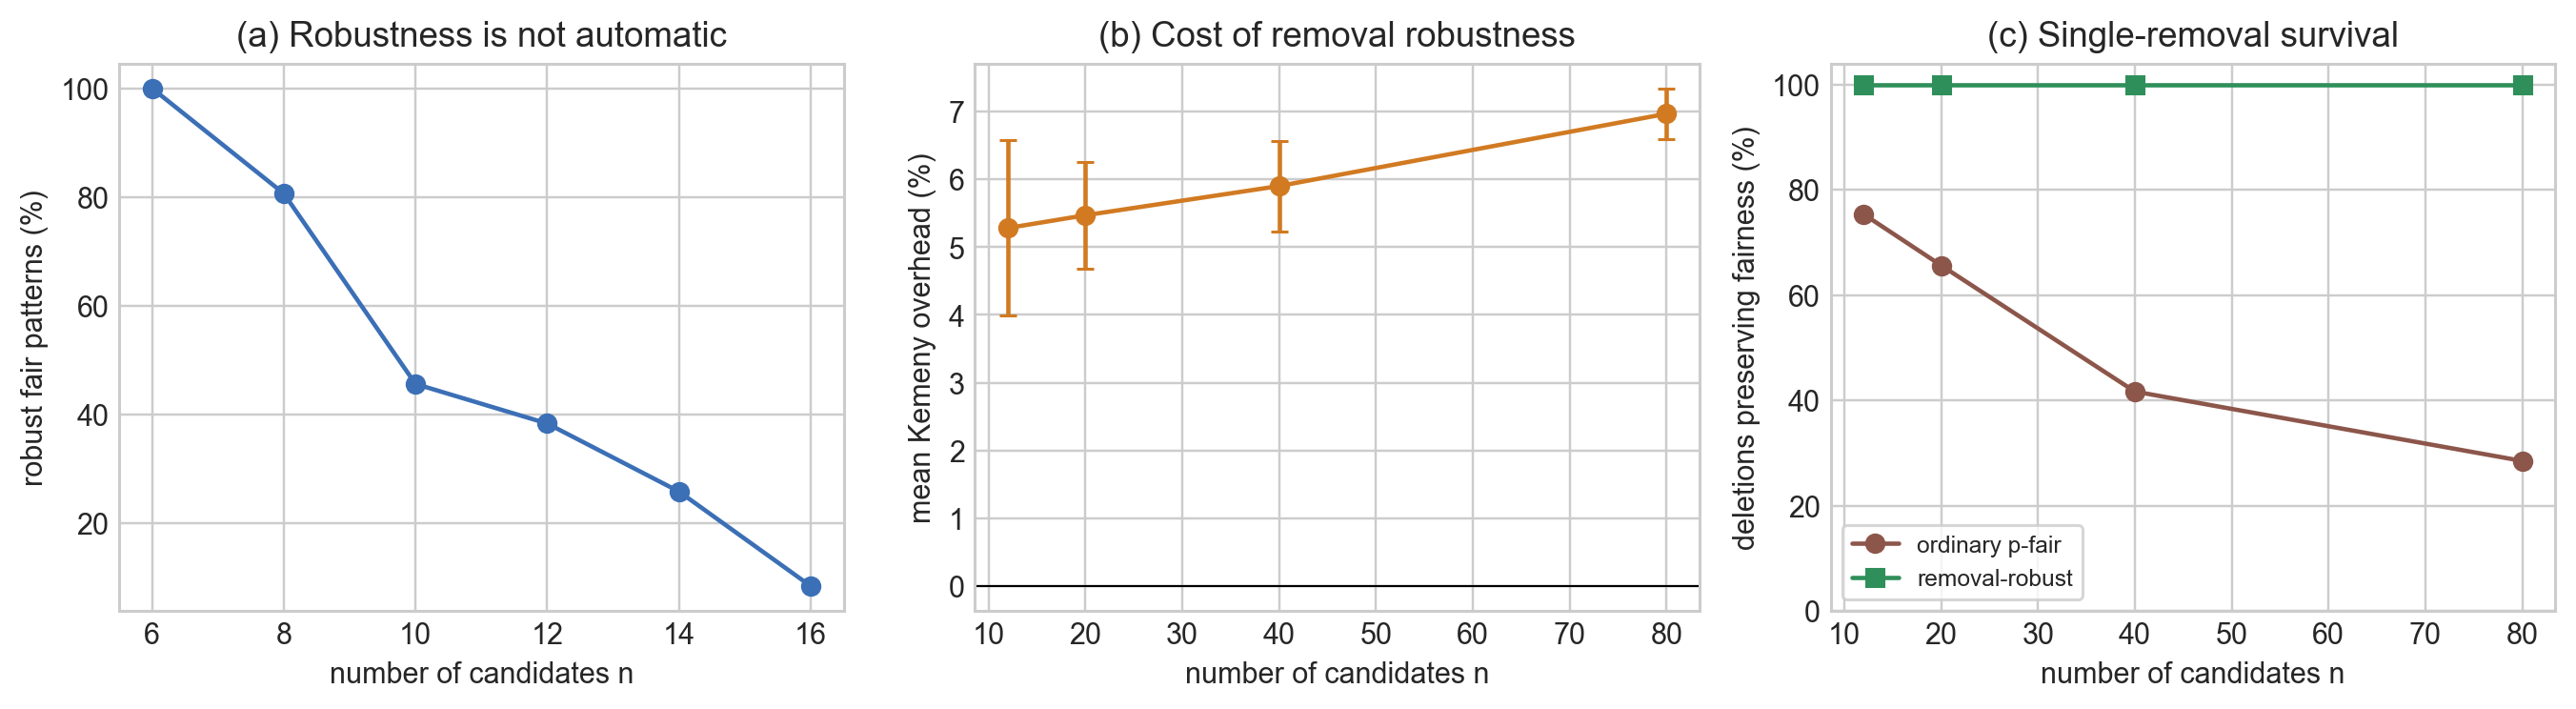
\includegraphics[width=\textwidth]{fig_removal_robustness.png}
  \caption{Results from the small tests.  Panel (a) shows the percentage of
  p-fair patterns that survived every removal.  Panel (b) shows the average
  percentage cost difference between the robust and p-fair algorithms; the
  small vertical bars show the standard error across 24 trials.  Panel (c)
  shows how often each algorithm's output stayed p-fair after one candidate
  was removed.}
  \label{fig:removal-robustness}
\end{figure}

First, we counted how many p-fair patterns survived every removal.  For each
$n$, the percentage combines group sizes $a=1,\ldots,n-1$.

\begin{center}
\begin{tabular}{@{}rrrrrrr@{}}
\toprule
$n$ & 6 & 8 & 10 & 12 & 14 & 16 \\
\midrule
robust among p-fair & 100\% & 80.65\% & 45.61\% & 38.34\% & 25.83\% & 8.45\% \\
\bottomrule
\end{tabular}
\end{center}

Every p-fair pattern happened to survive when $n=6$, but only 8.45\% survived
when $n=16$.  Thus p-fairness by itself did not guarantee removal robustness
in this test.

The next table shows the average results for the computer-made rankings.  Each
row is based on 24 trials.

\begin{center}
\begin{tabular}{@{}rrrr@{}}
\toprule
$n$ & cost difference & p-fair survival & robust survival \\
\midrule
12 & 5.28\% & 75.35\% & 100\% \\
20 & 5.47\% & 65.63\% & 100\% \\
40 & 5.90\% & 41.67\% & 100\% \\
80 & 6.97\% & 28.49\% & 100\% \\
\bottomrule
\end{tabular}
\end{center}

Across the trials, the average percentage cost difference between the two
algorithms was about 5.3\% to 7.0\%.  This is only a comparison of these two
algorithms, not the exact cost of adding robustness.  The robust answers
survived every removal, as required.  For the four sizes we tested, p-fair
survival went from 75.35\% down to 28.49\%.

For the small $n=7$ tests, we divided our algorithm's cost by the cost of the
best robust ranking.  A result of 1 would mean that our algorithm found the
best answer exactly.  The average was 1.049 and the largest was 1.147 over the
24 tests.  These examples do not change the proved bound of 3.  They only show
what happened in this small experiment.

For the Sushi example, the p-fair answer had Kemeny cost 2,574 and survived
50\% of the possible single-item removals.  The robust answer had cost 2,758
and survived every removal.  Its cost was 7.15\% higher in this example.

\section{Related work}

We found several ideas that are close to ours.  Wei et al.~\cite{wei2022}
studied proportionately fair rank aggregation when the candidate set does not
change.  Hottenrott et al.~\cite{hottenrott2021} studied planned car sequences
when an item fails.  Israel and Brill~\cite{israel2025} allow a proportional
ranking to be recalculated while alternatives are selected.  Ando and
Yokoi~\cite{ando2026} studied a more general mathematical model for prefix
rules and for finding a closest ranking.

As far as we could tell, none of these papers studies our exact condition:
one published two-group p-fair ranking must stay p-fair after any single
candidate is removed, without rearranging the remaining candidates.  We did
not find earlier work on that exact question.

Our question is narrow.  We study two groups and only one removal.  In this
setting, we prove that a robust pattern always exists and show how to find a
closest robust ranking to one input.  We are not claiming that robust
sequences in general are new.

\section{Conclusion}

A ranking can be p-fair and still break when one candidate leaves.  For two
groups, we can avoid this problem before publishing the list.  The proof is
mostly careful prefix counting, and it gives a linear algorithm.  We can also
find the closest robust ranking and use it inside a known aggregation method.
The model is small, but it shows that fairness and stability are not the same
thing.

There are still many things this paper does not solve.  It only handles two
groups, one removal, complete rankings, and group labels that are known and
correct.  We dont know from this paper if the same pattern can survive two
removals.  We also dont prove that a removal-robust pattern always exists for
three or more groups.  These are possible questions to study later.

\begin{thebibliography}{9}

\bibitem{ando2026}
S.~Ando and Y.~Yokoi.
Ranking and rank aggregation with matroid prefix constraints.
\emph{arXiv:2607.07153}, 2026.

\bibitem{chakraborty2025}
D.~Chakraborty, H.~Das, S.~Dey, and A.~H.~Y.~Yan.
Improved rank aggregation under fairness constraint.
In \emph{IJCAI}, 2025.

\bibitem{dwork2001}
C.~Dwork, R.~Kumar, M.~Naor, and D.~Sivakumar.
Rank aggregation methods for the Web.
In \emph{Proceedings of the 10th International World Wide Web Conference},
pages 613--622, 2001.

\bibitem{hottenrott2021}
A.~Hottenrott, L.~Waidner, and M.~Grunow.
Robust car sequencing for automotive assembly.
\emph{European Journal of Operational Research}, 291(3):983--994, 2021.

\bibitem{israel2025}
J.~Israel and M.~Brill.
Dynamic proportional rankings.
\emph{Social Choice and Welfare}, 64:221--261, 2025.

\bibitem{mattei2013}
N.~Mattei and T.~Walsh.
PrefLib: A library for preferences.
In \emph{Algorithmic Decision Theory}, 2013.

\bibitem{wei2022}
D.~Wei, M.~R.~Islam, B.~Schieber, and S.~Basu Roy.
Rank aggregation with proportionate fairness.
In \emph{ACM SIGMOD}, 2022.

\end{thebibliography}

\end{document}
